\documentclass[10pt,a4paper,twoside]{article}
\usepackage[dutch]{babel}
%laad de pakketten nodig om wiskunde weer te geven :
\usepackage{amsmath,amssymb,amsfonts,textcomp}
%laad de pakketten voor figuren :
\usepackage{graphicx}
\usepackage{float,flafter}
\usepackage{hyperref}
\usepackage{inputenc}
\usepackage{algorithm}
\usepackage{algpseudocode}
%zet de bladspiegel :
\setlength\paperwidth{20.999cm}\setlength\paperheight{29.699cm}\setlength\voffset{-1in}\setlength\hoffset{-1in}\setlength\topmargin{1.499cm}\setlength\headheight{12pt}\setlength\headsep{0cm}\setlength\footskip{1.131cm}\setlength\textheight{25cm}\setlength\oddsidemargin{2.499cm}\setlength\textwidth{15.999cm}

\begin{document}
\begin{center}
\hrule

\vspace{.4cm}
{\bf {\Huge Problem 3}}
\vspace{.2cm}
\end{center}
{\bf Name: Cheng Chen}  \\
{\bf ID:40222770}\\
{\bf function: tan(x)}\\
{\bf Concordia University}\\
{\bf SOEN 6011: Software Engineering Processes} {\bf  } \hspace{\fill}  17 July  2022 \\
\hrule
%\bf genereert vette letters, \large \Large \huge \Huge \tiny \small ... verschillende lettergroottes, met \em, \it, \sl krijg je cursieve tekst
%Je moet accolades gebruiken om aan te geven waarop je het commando precies wil laten inwerken.
% commentaar zet je in de tex-file met een %-tekentje voor.



%de ~ zorgt ervoor dat het ! met een spatie aan de tekst wordt geplakt en niet naar de volgende lijn verhuist.  Omdat latex na elk . automatisch een dubbele spatie invoegt, kan je ~ ook gebruiken om te voorkomen dat je na een afkorting bvb.~een dubbele spatie krijgt.

%1 open lijn wordt door latex gewoon als spatie gezien, met twee linefeeds  begint een nieuwe paragraaf.  Als je wil voorkomen dat de tekst inspringt, kan je het commando \noindent gebruiken.  \\ springt naar een volgende lijn, \newpage naar een volgend blad.


%\begin{figure}
%\centering
%\includegraphics[width=0.7\linewidth]{figje}
%\caption{}
%\label{fig:figje}
%\end{figure}
\section{Mindmap}
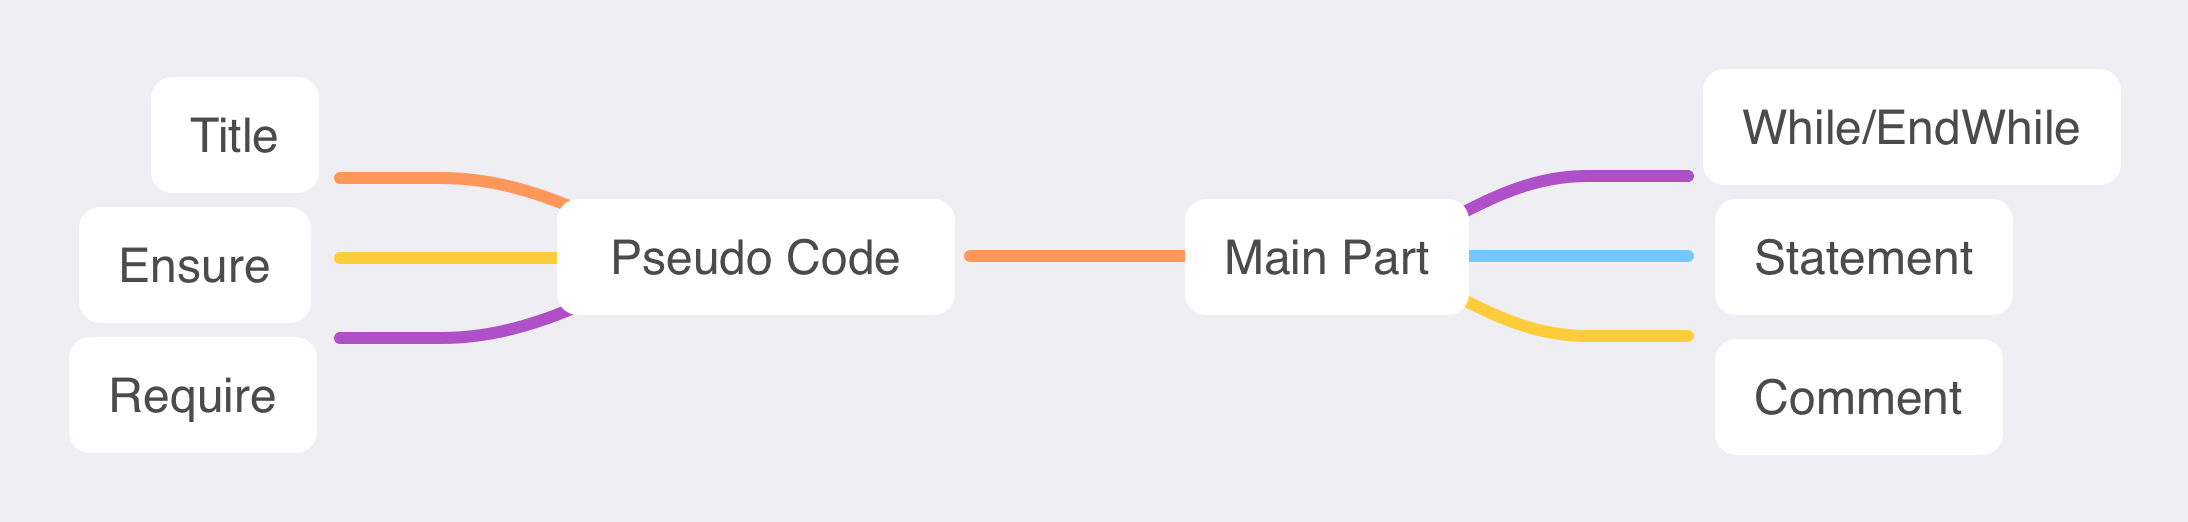
\includegraphics[scale=0.6]{problem3MindMap.png}

\section{Algorithm 1}
%Met het commando \sectie{naamtitel} maak je een nieuwe titel aan.
\subsection{Description}

Algorithm 1 is based on the taylor series of $tan(x)$. ($tan(x) = x + 1/3\times x^3 +2/15 \times x^5 + ...$
). This formula is used to calculate the approximation of $tan(x)$.

\subsection{Technical reasons}

\begin{itemize}
    \item advantages:Since the taylor series is a hard coded formula, it is easy to implement. 
    \item disadvantages:Since it's impossible to include all items in the full taylor serie of $tan(x)$, the result is an approximation, not the real result. What can be done is to include as more items as possible to increase the accuracy.
\end{itemize}

\subsection{Pseudo code}
\begin{algorithm}
\caption{Implementation}\label{alg:cap}
\begin{algorithmic}
\Require $x \in R, x\neq \pi/2 +k\times\pi$
\Ensure x is real number, if not, ask the user to input again
\State \bf{Start}
\State make x between 1.57 and -1.57
\While{True}
    \State $x \gets input$
    \State $y \gets x+x^3/(1\times3)+(2\times x^5)/(1\times3\times5$)
    \State \bf{output} $y$
\State end while if user exits the program
\EndWhile
\end{algorithmic}
\end{algorithm}

%hier werd verwezen naar de tabel die als \label (naam} 'tabel1' kreeg.



\section{Algorithm 2}
%Met het commando \sectie{naamtitel} maak je een nieuwe titel aan.
\subsection{Description}

Algorithm 2 uses the value of $tan(0.01)$ and $tan(a+b)=(tan(a)+tan(b))/(1-tan(a)*tan(b))$. The input $x$ will be separated by 0.01 for the calculation. For example, $tan(0.01+0.01)=(tan(0.01)+tan(0.01))/(1-tan(0.01)*tan(0.01))$, then $tan(0.02)$ can be calculated. Therefore it can be easily conducted that $tan(0.03), tan(0.04) and ...$ can be calculated.

\subsection{Technical reasons}

\begin{itemize}
    \item advantages:Since the $tan(x)$ in algorithm 2 is calculated according to $tan(a+b)=(tan(a)+tan(b))/(1-tan(a)*tan(b))$, the output is closer to the real $tan(x)$ than algorithm 1.
    \item disadvantages:First, every input $x$ will be separated by 0.01 one by one, it takes more time than algorithm 1 to calculate $tan(x)$. Second, the problem of accuracy also exists. If the user input a $x$ like 0.0003 or 12.384727. Algorithm 2 can just calculate them as $tan(0.00)$ or $tan(12.39)$. The more accuracy it is (like being separated by $0.0001$ or a smaller number), the more time it takes. Therefore, the number to be used for separated here is 0.01.
\end{itemize}

\subsection{Pseudo code}
\begin{algorithm}
\caption{Implementation}\label{alg:cap}
\begin{algorithmic}
\Require $x \in R$
\Ensure x is real number, if not, ask the user to input again
\State \bf{Start}
\State make x between 1.57 and -1.57
\While{True}
    \State $x \gets input$
    \State $out \gets 0$;
        \While{$x>0$}
            \State out= (out+0.010000333346667207)/(1-out*0.010000333346667207)
            \State x-=0.01
        \EndWhile
    \State $y \gets out$
    \State \bf{output} $y$
\State end while if user exits the program
\EndWhile
\end{algorithmic}
\end{algorithm}




%met enumerate genereer je een opsomming, itemize maakt verschillende puntjes

\end{document}
